\documentclass[12pt,enlgish,openany,twoside,letterpaper]{book}

%Muestra los márgenes del documento para evitar Warnings
%Para activar la siguiente línea quite el simbolo % 
%\usepackage[showframe]{geometry}

%Usando el paquete BibLaTeX
%Cita normal con \cite[página]{} y cita con paréntesis \parencite[página]{}

% Configuración de BibLaTeX
%\usepackage[backend=biber,style=authoryear,maxcitenames=2,maxbibnames=99,giveninits=true,uniquename=false]{biblatex}
%\addbibresource{biblio.bib}

% Personalizar el formato de las citas y la bibliografía
%\DeclareNameAlias{sortname}{family-given}
%\DeclareDelimFormat{multinamedelim}{\addcomma\space}
%\DeclareDelimFormat{finalnamedelim}{\addcomma\space\&\space}
%\DeclareFieldFormat{titlecase}{\MakeSentenceCase*{#1}}
%\DeclareFieldFormat[article,inbook,incollection,inproceedings,patent,thesis,unpublished]{title}{\titlecase{#1}}
%\DeclareFieldFormat{journaltitlecase}{\titlecase{#1}}
%\DeclareFieldFormat{pages}{#1}
%\DeclareFieldFormat{volume}{\mkbibbold{#1}}
%\renewbibmacro{in:}{}
%\AtEveryBibitem{\clearfield{month}}

\usepackage[spanish]{babel}
\usepackage[utf8]{inputenc}
% Carácteres especiales
\usepackage{fontenc}
% More advance packages

\usepackage{amssymb,amsbsy,mathrsfs,rotating,float,multirow,upgreek,amsmath,lineno,bm}
\usepackage{breakcites}
\usepackage{listings}
\usepackage{pgfplots}
\usepackage{tikz}
\usepgfplotslibrary{groupplots}
\usepackage{longtable}
\setlength{\LTcapwidth}{6in}
\usepackage[utf8]{inputenc}
\usepackage{epsfig,epic,eepic,threeparttable,amscd,here,lscape,tabularx,graphicx }
\usepackage{booktabs}
\usepackage{tabu,array}
\usepackage{overpic}
\usepackage{microtype}
%%%%%%%%%%%
%\usepackage{newtxtext,newtxmath}
%%%%%%%%%%%
%\usepackage[table]{xcolor}
\usepackage{caption}
\usepackage{subcaption}
% Permite ver y configurar los parámetros de la página
\usepackage{layout}
%Hyperref permite ver las secciones del texto
\usepackage[hidelinks]{hyperref}
\usepackage{cleveref}
\usepackage{lmodern}
\usepackage{nomencl}
\usepackage[T1]{fontenc}
%% This code creates the groups
% -----------------------------------------
\renewcommand{\nomname}{\sffamily List of Symbols and Abbreviations} 

\usepackage{etoolbox}
\renewcommand\nomgroup[1]{%
  \item[\Large\bfseries
  \ifstrequal{#1}{A}{Number Sets}{%
  \ifstrequal{#1}{B}{Symbols}{%
  \ifstrequal{#1}{C}{Abbreviations}{}}}%
]\vspace{10pt}}
\makenomenclature
% -----------------------------------------

\newcommand{\todo}[1]{\textcolor[rgb]{1.00,0.00,0.00}{#1}}




\providecommand{\var}[1]{{\ensuremath{var}}\{#1\}}
\DeclareMathOperator{\tire}{\negthinspace-\negthinspace}
\DeclareRobustCommand{\legend}[1]{%
	\textcolor{#1}{\rule{1ex}{2ex}}%
}
\newcommand{\lineplot}[1]{
	\textcolor{#1}{\rule{1.5ex}{0.3ex}}%
}

%%%% custom colors
\colorlet{color0}{blue!40!gray}% pearson *
\colorlet{color1}{blue!80!gray} %pearson **
\colorlet{color2}{red!40!gray} %n-pearson*
\colorlet{color3}{red!80!gray}%n-pearson**
\colorlet{color4}{green!40!gray} %plv*
\colorlet{color5}{green!80!gray} 

\definecolor{frontal}{RGB}{141, 211, 199}
\definecolor{frontal_left}{RGB}{255, 237, 111}
\definecolor{frontal_right}{RGB}{255, 255, 179}
\definecolor{central_right}{RGB}{251, 128, 114}
\definecolor{central_left}{RGB}{204, 235, 197}
\definecolor{posterior_right}{RGB}{253, 180, 98}
\definecolor{posterior_left}{RGB}{217, 217, 217}
\definecolor{posterior}{RGB}{179, 222, 105}


%%%%
\definecolor{darkorange25512714}{RGB}{255,127,14}
\definecolor{forestgreen4416044}{RGB}{44,160,44}
\definecolor{steelblue31119180}{RGB}{31,119,180}
%%%%

\newcommand{\Objectiveonename}{}
\newcommand{\Objectivetwoname}{}
\newcommand{\Objectivethreename}{}

%% defining objective names
\renewcommand{\Objectiveonename}{Develop a neural networks-based optimization strategy that is adaptable to different noise levels and specific restrictions, ensuring results comparable to conventional optimization techniques in terms of compliance with resSingle-trial kernel-based functional connectivity for enhanced feature extriactions and robustness in EEG-based MI-BCI}
\renewcommand{\Objectivetwoname}{
Develop a customized neural networks-based non-linear programming optimization scheme for gas-powered energy systems that considers physical limits and non-differentiable functions, focusing on modeling gas supply behavior and compliance with system constraintsKCS-FCnet: Kernel Cross-Spectral Functional Connectivity Network for automatic EEG representation in MI-BCI}
\renewcommand{\Objectivethreename}{Develop a customized neural networks-based non-linear programming optimization strategy for the Colombian gas-powered energy system, modeling the behavior of supply-demand flows and pressures and incorporating physical boundaries and non-differentiable functions that ensure efficiency over time and convergencequalitative and quantitative post-hoc and intrinsic interpretation for MI-BCI models}

%%%


% Create author commands
\newcommand{\studentname}{}
\newcommand{\submissiondate}{}
\newcommand{\academictitle}{}
\newcommand{\resgroupone}{}
%\newcommand{\resgrouptwo}{}
\newcommand{\researchtopic}{}
\newcommand{\thesisname}{}
\newcommand{\director}{}
\newcommand{\codirector}{}
\newcommand{\issuedate}{}
\newcommand{\palabrasclave}{}
\newcommand{\keywords}{}
\newcommand{\schlusselworter}{}
\newcommand{\palavraschave}{}
\newcommand{\sede}{}
\newcommand{\department}{}
\newcommand{\faculty}{}

%Información de la tesis
%Diligenciar aquí los datos para su carga automática donde se requiera en el documento
\renewcommand{\studentname}{Julian Andres Salazar Parias}
\renewcommand{\thesisname}{Low-Latency EEG Marker Integration in Serious Games for Neurocognitive Assessment}
\renewcommand{\issuedate}{2025}
\renewcommand{\submissiondate}{2025}
\renewcommand{\director}{MSc Bernardo Andrés Cardona Noreña}
\renewcommand{\academictitle}{Maestría en ingeniería - Automatización Industrial}
\renewcommand{\resgroupone}{Grupo de Control y Procesamiento Digital de Señales (GCPDS) }
%\renewcommand{\resgrouptwo}{}
\renewcommand{\researchtopic}{Inteligencia Artificial}
\renewcommand{\sede}{Manizales} 
\renewcommand{\department}{Departamento de ingeniera eléctrica, electrónica y computación}
\renewcommand{\faculty}{Facultad de ingeniera y arquitectura}


%Palabras clave del documento - Tener presente los Theasurus https://www.thesaurus.com/
%Disponible en 3 idiomas aunque se puede extender a francés o otro idioma

\renewcommand{\palabrasclave}{Use palabras clave que estén en Theasaurus} 
\renewcommand{\keywords}{Use keywords available in Theasaurus}

% Estilo de los encabezados y pies de página
\usepackage{fancyhdr}

\fancyhf{}%
\pagestyle{fancyplain}
\textheight22.5cm \topmargin0cm \textwidth16.5cm \headheight22pt
\oddsidemargin0.5cm \evensidemargin-0.5cm%
\fancypagestyle{plain}{
\fancyhead[RO,LE]{}
\fancyhead[RE,LO]{\small \textbf{\thesisname}}
\fancyfoot[CO,CE]{\thepage}
}
\pagestyle{fancy}
\fancyhf{}% Clear all header and footer fields
\renewcommand{\chaptermark}[1]{\markboth{\thechapter.\; #1}{}}
% \renewcommand{\sectionmark}[1]{\markright{\thesection.\; #1}{}} % Comentado para no usar secciones en encabezados
\fancyhead[LO,RE]{\leftmark} % Pone el nombre del capítulo en el encabezado izquierdo de las páginas impares y en el derecho de las páginas pares
% \fancyhead[RO,LE]{\rightmark} % Comentado para no poner nombre de sección en el encabezado
\fancyfoot[CO,CE]{\thepage} % Pone el número de página en el centro del pie de página
\thispagestyle{fancy}% Ensure that the first page of each chapter will have headers and footers as well



\usepackage{titlesec}
% Permite personalizar los títulos de sección y de capítulos
% hang lo deja en el mismo renglón, display lo despliega
% Elimina el "Capitulo" y deja solo el número

\titleformat{\chapter}[hang]
  {\sffamily\Huge\bfseries}{\thechapter}{0.5cm}{\sffamily\Huge}
\titleformat{\section}[hang]{\sffamily\LARGE}{\thesection}{0.5cm}{}
\titleformat{\subsection}[hang]{\sffamily\Large}{\thesubsection}{0.5cm}{}
\titleformat{\subsubsection}[hang]{\sffamily\large}{\thesubsubsection}{0.5cm}{}
\titleformat{\paragraph}[runin]{\sffamily\normalsize}{}{}{\emph}

%Coloca anexo o apéndice en la Tabla de contenido
\usepackage[toc,page]{appendix}

% Configuración de las páginas en twoside-mode
% Permite ver y configurar los parámetros de la página
\setlength{\voffset}{-0.25in}
\setlength{\headwidth}{467pt}
\setlength{\headheight}{22pt}
\setlength{\oddsidemargin}{0pt}
\setlength{\evensidemargin}{0pt}
\setlength{\marginparwidth}{0pt}
\setlength{\marginparsep}{0pt}
\setlength{\parskip}{2em}
\setlength{\footskip}{20pt}
\setlength{\textheight}{650pt}
\setlength{\textwidth}{467pt}
\setlength{\headsep}{5pt}
\setlength{\parindent}{0pt}
\setlength{\baselineskip}{10pt plus 5pt minus 5pt}
\renewcommand{\theequation}{\thechapter-\arabic{equation}}
\renewcommand{\thefigure}{\textbf{\thechapter-\arabic{figure}}}
\renewcommand{\thetable}{\textbf{\thechapter-\arabic{table}}}

%Define la distancia de la primera linea de un parrafo a la margen
\parindent0cm 

%Espacio entre lineas
\renewcommand{\baselinestretch}{1}

%Para rotar texto, objetos y tablas seite.
\usepackage{rotating}

%Permite incluir mecanismos y reacciones químicas
\usetikzlibrary{positioning}
\usetikzlibrary{mindmap}
\usepackage{chemformula}
\usepackage{chemfig}
\usepackage{xcolor}

\usetikzlibrary{calc,arrows.meta}% per right to e left to
\tikzset{
myedge/.style={->, -{Latex[#1]}}
}

%Fuente de la presentación Ancizar Sans UNAL
%Para usar este compilado en Overleaf se debe usar el compilador XeLaTeX o LuaLaTeX!!
%Menu -> Compiler -> XeLaTeX o LuaLaTeX
%La siguiente línea debe comentarse si desea compilar con pdfLaTeX
%\RequireXeTeX

% Definición de la fuente Ancizar Sans
\newif\ifxetexorluatex

\ifxetexorluatex
  \usepackage{fontspec}
  \usefonttheme{serif}
  \setmainfont{AncizarSans}[Path=./AncizarSans/,Scale=1,Extension=.otf,UprightFont=*-Regular,BoldFont=*-Bold,ItalicFont=*-Italic,BoldItalicFont=*-BoldItalic]
\else
  % Si se compila con pdfLaTeX, cargar la fuente apropiada aquí
  \usepackage[T1]{fontenc}
\fi
% Metadatos del documento
\AtBeginDocument{%
	\hypersetup{
		pdfborder={0 0 0},
		pdfauthor={\studentname},
		pdfsubject={\thesisname}, 
		pdfcreator={\studentname},
		pdfproducer={\studentname},
	}
}

%Carga el simbolo de grado y el de Angstrom
\newcommand{\angstrom}{\textup{\AA}}
\newcommand{\grad}{$^{\circ}$}

\newtheorem{theorem}{Theorem}
\newtheorem{lemm}[theorem]{Lemma}
\newtheorem{proof}{Proof}[theorem]
\newtheorem{propo}[theorem]{Proposition}

\usepackage[acronym=true, 
            toc=true, 
            numberline=false, 
            nopostdot=true, 
            section=chapter, 
            nomain=true]{glossaries-extra}
\setabbreviationstyle[acronym]{long-short}
\renewcommand{\glsnamefont}[1]{\textsc{\normalfont\large\bfseries #1}}
\glssetcategoryattribute{acronym}{hyperoutside}{false}
%Inicio del documento, no olvide la etiqueta de cierre al final \end{document}
%\newglossary*{symbols}{List of Symbols}
\newglossary[slg]{symbols}{not}{ntn}{Symbols}


\newglossaryentry{ip}
{
  name={IP},
  description={Inner Point},
  type=acronym,
  sort={ip}
}
\newglossaryentry{pi}
{
  name={\ensuremath{\pi}},
  description={ratio of circumference of circle to its
               diameter},
  type=symbols,
  sort={pi}
}
\newglossaryentry{upme}
{
  name={UPME},
  description={Unidad de Planeación Minero Energética},
  type=acronym,
  sort={upme}
}

\newglossaryentry{creg}
{
  name={CREG},
  description={Comisión de Regulación de Energía y Gas},
  type=acronym,
  sort={creg}
}

\newglossaryentry{ai}
{
  name={AI},
  description={Artificial Intelligence},
  type=acronym,
  sort={ai}
}
\newglossaryentry{gcpds}
{
  name={GCPDS},
  description={Grupo de Control  y Procesamiento Digital de Señales},
  type=acronym,
  sort={gcpds}
}
\newglossaryentry{sni}
{
  name={SNI},
  description={Sistema Nacional Interconectado},
  type=acronym,
  sort={sni}
}

\newglossaryentry{lp}
{
  name={LP},
  description={Linear Programming},
  type=acronym,
  sort={lp}
}
\newglossaryentry{pevi}
{
  name={PEVI},
  description={Programa de Evaluación Industrial},
  type=acronym,
  sort={pevi}
}

\newglossaryentry{qp}
{
  name={QP},
  description={Quadratic Programming},
  type=acronym,
  sort={qp}
}

\newglossaryentry{sdp}
{
  name={SDP},
  description={Semi-Defined Programming},
  type=acronym,
  sort={sdp}
}


\newglossaryentry{socp}
{
  name={SOCP},
  description={Second-Order Cone Programming},
  type=acronym,
  sort={socp}
}
\newglossaryentry{mip}
{
  name={MIP},
  description={Mixed-Integer Programming},
  type=acronym,
  sort={mip}
}

\newglossaryentry{ann}
{
  name={ANN},
  description={Artificial Neural Networks},
  type=acronym,
  sort={ann}
}
\newglossaryentry{dnn}
{
  name={DNN},
  description={Deep Neural Networks},
  type=acronym,
  sort={dnn}
}
\newglossaryentry{gnn}
{
  name={GNN},
  description={Graph Neural Networks},
  type=acronym,
  sort={gnn}
}

\newglossaryentry{pinn}
{
  name={PINN},
  description={Physics-Informed Neural Network},
  type=acronym,
  sort={pinn}
}
\newglossaryentry{nlp}
{
  name={NLP},
  description={Non-Lineal Programming},
  type=acronym,
  sort={nlp}
}
\newglossaryentry{nn}
{
  name={NN},
  description={Neural Networks},
  type=acronym,
  sort={nn}
}
\newglossaryentry{ad}
{
  name={AD},
  description={Automatic Differentiation},
  type=acronym,
  sort={ad}
}
\newglossaryentry{mape}
{
  name={MAPE},
  description={Mean Absolute Percentage Error},
  type=acronym,
  sort={mape}
}
\newglossaryentry{iqr}
{
  name={IQR},
  description={Interquartile Range},
  type=acronym,
  sort={iqr}
}

\newglossaryentry{mse}
{
  name={MSE},
  description={Mean Squared Error},
  type=acronym,
  sort={mse}
}
\newglossaryentry{mae}
{
  name={MAE},
  description={Mean Absolute Error},
  type=acronym,
  sort={mae}
}
\newglossaryentry{cvxpy}{
name={CVXPY},
description={Convex Optimization in Python},
type=acronym,
sort={cvxpy}
}

\makeglossaries
\usepackage{glossaries}
\makeglossaries

\usepackage{graphicx}


\newacronym{CREG}{CREG}{Comisión de Regulación de Energía y Gas}
% Abbreviations
\usepackage[acronym=true, 
            toc=true, 
            numberline=false, 
            nopostdot=true, 
            section=chapter, 
            nomain=true]{glossaries-extra}
\setabbreviationstyle[acronym]{long-short}
\renewcommand{\glsnamefont}[1]{\textsc{\normalfont\large\bfseries #1}}
\glssetcategoryattribute{acronym}{hyperoutside}{false}

























\begin{document}



%% math comands

% custom commands
\providecommand{\ppunto}[2]{\langle#1, #2 \rangle}% producto punto
\providecommand{\promed}[1]{{\mathbb{E}}\left\lbrace #1\right\rbrace}% operador de promedio
\providecommand{\promeddd}[2]{\mathbb{E}_{#1}\!\left\{#2\right\}}% op{\tiny }erador de promedio
\providecommand{\promedd}[2]{\mathds{E}_{#1}\left\{#2\right\}}% operador de promedio
\providecommand{\cov}[2]{{\fam=7 cov}\{#1, #2\}}% operador de covarianza
\providecommand{\gaus}[2]{{\fam=6 N}(#1 #2)} % FDP Gauss
% Kronecker delta function
\providecommand{\Kronecker}[2]{\delta_{K}( #1 , #2 )}
% cardinality
\providecommand{\Cardinality}[1]{| #1 |}



\providecommand{\est}[1]{{\widetilde {#1}}}
\providecommand{\s}[1]{\negthickspace#1\negthickspace}%
\newcolumntype{C}[1]{>{\centering}m{#1}}
\newcommand{\subconj}{\negthinspace\subset\negthinspace }
\newcommand{\en}{\negthinspace\in\negthinspace }
\newcommand{\igual}{\negthinspace=\negthinspace}
\newcommand{\dos}{\negthinspace:\negthinspace}

\newcommand{\Real}{\mathbb{R}}
\newcommand{\Natural}{\mathbb{N}}

\newcommand{\Tr}[1]{Tr \left( #1 \right)}
\newcommand{\diag}[1]{diag \left( #1 \right)}

\newcommand{\func}[1]{\mathcal {#1}}

\newcommand{\ve}[1]{\bm {#1}}
\newcommand{\mat}[1]{\bm {#1}}
%\providecommand{\ve}[1]{{\mathbf {#1}}} %
%\providecommand{\mat}[1]{{\mathbf {#1}}} %

\newcommand{\x}{\negthickspace\times\negthickspace}

%%

%Nombres y formatos de títulos, tablas y figuras
%Use \sffamily para dejar con letra Sans Serif, sin etiqueta queda LaTeX clásico
\renewcommand{\listfigurename}{\sffamily Lista de Figuras}
\renewcommand{\listtablename}{\sffamily Lista de Tablas}
\renewcommand{\contentsname}{\sffamily Content}
\renewcommand{\chaptername}{\sffamily Chapter}
\renewcommand{\tablename}{\scriptsize \centering \textbf{Table}}
\renewcommand{\figurename}{\scriptsize \centering \textbf{Figure}}
\renewcommand{\appendixname}{\sffamily Appendix}

%Cambia el nombre de la sección de referencias
\renewcommand{\bibname}{\sffamily References}

%Páginas de Presentación del documento - No modificar esto se hace automáticamente
{\newpage
\thispagestyle{empty}
\begin{center}
\begin{figure}
\centering

\epsfig{file=Figures/EscudoUN2016,scale=1}%
\end{figure}
\vspace{2.5cm}
\textbf{\Huge \thesisname} \\ 
\vspace{2.5cm}
\textbf{\Large \studentname} \\
\vspace{5.0cm}
\small Universidad Nacional de Colombia \\
\faculty \\
\department \\
\sede, Colombia\\
\issuedate
\newpage 
\thispagestyle{empty}
\vspace{2.5cm}
\textbf{\Huge \thesisname} \\
\vspace{2.5cm}
\textbf{\Large \studentname} \\
\vspace{2.5cm}
\small Tesis presentada como requisito parcial para optar por el título de: \\
{\bfseries \academictitle}\\
\vspace{2.5cm}
Director(a): \\
\director \\
% Codirector(a): \\
% \codirector \\
\vspace{2.5cm}
Línea de investigación: \\ 
\researchtopic\\
Grupo de investigación: \\
\resgroupone \\
%\resgrouptwo \\
\vspace{2.0cm} 
Universidad Nacional de Colombia \\
\faculty \\
\department \\
\issuedate
\end{center}

% Dedicatorias
\newpage
\thispagestyle{empty}
\begin{flushright}
\begin{minipage}{12.5cm}
\noindent
\\[10em]
%Modificar la cita que se quiere agregar
"The concern for man and his destiny must always be the primary interest of any technical effort. Never forget this between your diagrams and equations"
\\[3em]
\\ \textit{Albert Einstein}
\\[10em]
%Para anular la adición de una segunda cita anule las siguientes lineas desde acá mediante comentario (%)
"Believe you can, and you are halfway there."
\\[3em]
\\ \textit{Theodore Roosevelt}
%Hasta acá!
\end{minipage}
\end{flushright} 

% Declaracíon de originalidad del texto y del contenido
% No modificar, se hace automáticamente con los comandos ya definidos
\newpage
\chapter*{\sffamily Declaración}
\par Me permito afirmar que he realizado esta tesis de manera autónoma y con la única ayuda de los medios permitidos. Todos los pasajes que se han tomado de manera textual o figurativa de textos publicados y no publicados, los he reconocido en el presente trabajo. Ninguna parte del presente trabajo se ha empleado en ningún otro tipo de tesis.
\\[1em]
\sede, \submissiondate
\\[6em]
\rule{6cm}{0.5pt}\\
\studentname

}
%\begingroup
%\pagenumbering{roman}
       % Abbreviations
%\printglossary[type=\acronymtype, title=Abbreviations]
%\glsresetall
%\cleardoublepage
%\endgroup

{\pagestyle{plain} \pagenumbering{roman}
\setlength{\parskip}{1mm}
\chapter*{\sffamily Agradecimientos}
\addcontentsline{toc}{chapter}{Agradecimientos}


En primer lugar, quiero expresar mi más sincero agradecimiento a mis codirectores de tesis, el PhD Andrés Marino Álvarez Meza y el PhD César Germán Castellanos Domínguez, así como a mi director de tesis, el MSc Bernardo Andrés Cardona Noreña. Su orientación, conocimientos y compromiso fueron fundamentales para la realización de este trabajo. Gracias por su dedicación, paciencia y apoyo incondicional en cada etapa de este proceso.

Extiendo también mi profundo agradecimiento a mi familia, cuyo amor, comprensión y constante apoyo emocional me motivaron a superar cada desafío que enfrenté durante mi formación académica. Sin su respaldo, este logro no habría sido posible.

Finalmente, quiero reconocer al Grupo de Control y Procesamiento Digital de Señales por el apoyo académico brindado. Su colaboración y contribución fueron clave para el desarrollo de esta investigación. A todos ellos, gracias por formar parte de este camino y ayudarme a alcanzar esta meta.




\begin{flushright}
\studentname\\
\issuedate
\end{flushright}   
\include{Julian/abreviaciones}
\begingroup
%\pagenumbering{roman}
%\printglossary[type=\acronymtype, title=Abbreviations]
%\glsresetall
%\cleardoublepage
\endgroup
\include{Julian/abstraz ct}
\listoffigures
\addcontentsline{toc}{chapter}{Lista de figuras}
\listoftables 
\addcontentsline{toc}{chapter}{Lista de Tablas}
\tableofcontents 
\addcontentsline{toc}{chapter}{Contenido}
\clearpage
}

{\pagenumbering{arabic}
\setlength{\parskip}{\baselineskip}
%Incluir secciones del documento de aqui en adelante
%Use \include para incluir desde una página nueva e \input para incluir sin salto de página



\chapter{Preliminaries}\label{sec:preliminaries}

\section{Motivation}\label{sec:motivation}

Brain–Computer Interfaces (BCIs) have emerged as a powerful class of technologies that enable direct communication between the brain and external devices. These systems are increasingly being applied in neurorehabilitation, education, and clinical diagnosis due to their ability to monitor and interpret neural activity in real time. BCIs have the potential to revolutionize the way cognitive states are assessed and modulated by offering closed-loop interaction mechanisms that adapt to the user’s brain dynamics \cite{Lim2023,Lin2025}. Central to this capability is the choice of neuroimaging modality, which must meet strict criteria in temporal resolution, portability, and cost-effectiveness—especially in applications involving children or naturalistic settings.

Several neuroimaging techniques have been explored for use in Brain–Computer Interface (BCI) systems, each with distinct advantages and limitations. Functional Magnetic Resonance Imaging (fMRI) offers high spatial resolution and whole-brain coverage, but its cost, immobility, and dependence on specialized facilities make it impractical for real-time interaction or integration with everyday environments \cite{Yang2025}. Magnetoencephalography (MEG) provides excellent spatiotemporal resolution but is similarly constrained by high operational costs and the need for magnetically shielded rooms \cite{Peksa2023}. Functional Near-Infrared Spectroscopy (fNIRS), a more portable option, measures cortical hemodynamic responses with moderate spatial resolution and tolerance to movement \cite{Doherty2023}. However, its low temporal resolution limits its ability to capture fast-changing neural dynamics, such as those required for attentional monitoring or neurofeedback.

Electroencephalography (EEG), by contrast, emerges as the most suitable modality for BCI applications that demand real-time responsiveness, portability, and affordability. EEG records the brain's electrical activity through non-invasive scalp electrodes, offering millisecond-level temporal resolution ideal for tracking rapid cognitive events like attention shifts or inhibitory control. While EEG's spatial resolution is lower compared to fMRI or MEG, advances in signal processing—such as QEEG, functional connectivity analysis, and source localization—have greatly enhanced its ability to extract meaningful neurophysiological markers \cite{Caiado2025,Yadav2023, Varbu2022}. Moreover, EEG's lightweight hardware, low infrastructure requirements, and compatibility with embedded systems make it an ideal foundation for interactive, portable, and scalable BCI solutions.

\begin{figure}[h]
 \centering
 \includegraphics[width=1\textwidth]{Figures/Neuroimagrre.pdf}
 \caption{Comparison of neuroimaging modalities by spatial resolution, temporal resolution, and cost. EEG stands out for its affordability, portability, and millisecond-level responsiveness.}
 \label{fig:neuroimaging_comparison}
\end{figure}

One of the most compelling clinical applications of EEG-based BCIs is in the assessment and intervention of neurodevelopmental disorders such as Attention Deficit Hyperactivity Disorder (ADHD). ADHD affects approximately 10\% of children in Colombia \cite{salari2023global,pineda2003prevalence} and is characterized by persistent symptoms of inattention, hyperactivity, and impulsivity that interfere with academic performance, social relationships, and emotional regulation. Conventional diagnostic practices rely heavily on behavioral questionnaires and clinical observation, which, while informative, are inherently subjective and susceptible to bias \cite{raiker2017accuracy}. In this context, EEG offers a valuable alternative by enabling the objective measurement of neural correlates linked to attention and impulse control. Well-established EEG biomarkers such as elevated theta/beta ratios and altered event-related potentials (e.g., P300) have been extensively validated in the ADHD literature, making EEG a scientifically robust and clinically relevant tool for real-time cognitive monitoring and neurofeedback interventions.

Serious games are digital environments designed not solely for entertainment, but to fulfill educational, therapeutic, or cognitive objectives. In the context of neurodevelopmental disorders such as ADHD, they have become increasingly relevant as tools for both cognitive assessment and intervention \cite{Patino2025}. Their engaging and adaptive nature allows them to target specific executive functions—like attention, inhibition, and working memory—while maintaining high user motivation, particularly among children \cite{RodriguezTimana2024}. These features make serious games particularly compatible with EEG-based BCIs for interactive cognitive modulation.


Serious games designed for ADHD not only provide engaging environments for cognitive stimulation, but also serve as structured frameworks for assessing and training specific executive functions. Two principal paradigms guide the design of these games. The first is the task-based paradigm, which integrates classical neuropsychological tasks—such as the Go/No-Go, n-back, or Stroop test—into interactive game mechanics. This allows for the precise measurement of behavioral responses tied to well-established cognitive models \cite{Fang2025}. The second is the neurofeedback paradigm, in which the game dynamically responds to real-time EEG signals, offering auditory or visual feedback based on the user’s brain state. This paradigm supports operant conditioning mechanisms, encouraging users to self-regulate neural activity linked to attentional control and inhibition \cite{Firouzabadi2022}. 

These paradigms are often aligned with four core cognitive models critical to ADHD pathology: attention, working memory, inhibition, and planning. Games targeting the attentional model aim to improve sustained and selective attention, often requiring players to maintain focus amid distractions or shifting stimuli \cite{Chen2024}. Working memory is typically trained through tasks that require the temporary storage and manipulation of information, such as remembering sequences or updating mental representations. The inhibition model involves suppressing prepotent responses or resisting distractions—commonly implemented through fast-paced decision-making challenges or impulse control mechanics \cite{Takahashi2024, BreitlingZiegler2020}. Finally, the planning model emphasizes goal-directed behavior, encouraging users to sequence actions, solve multi-step problems, or anticipate future outcomes \cite{Lorini2022}. By aligning game mechanics with these cognitive models, serious games become powerful tools not only for engagement but for targeted neurocognitive intervention, particularly when combined with EEG-based BCIs that provide objective feedback on brain performance in real time.


\begin{figure}[h]
 \centering
 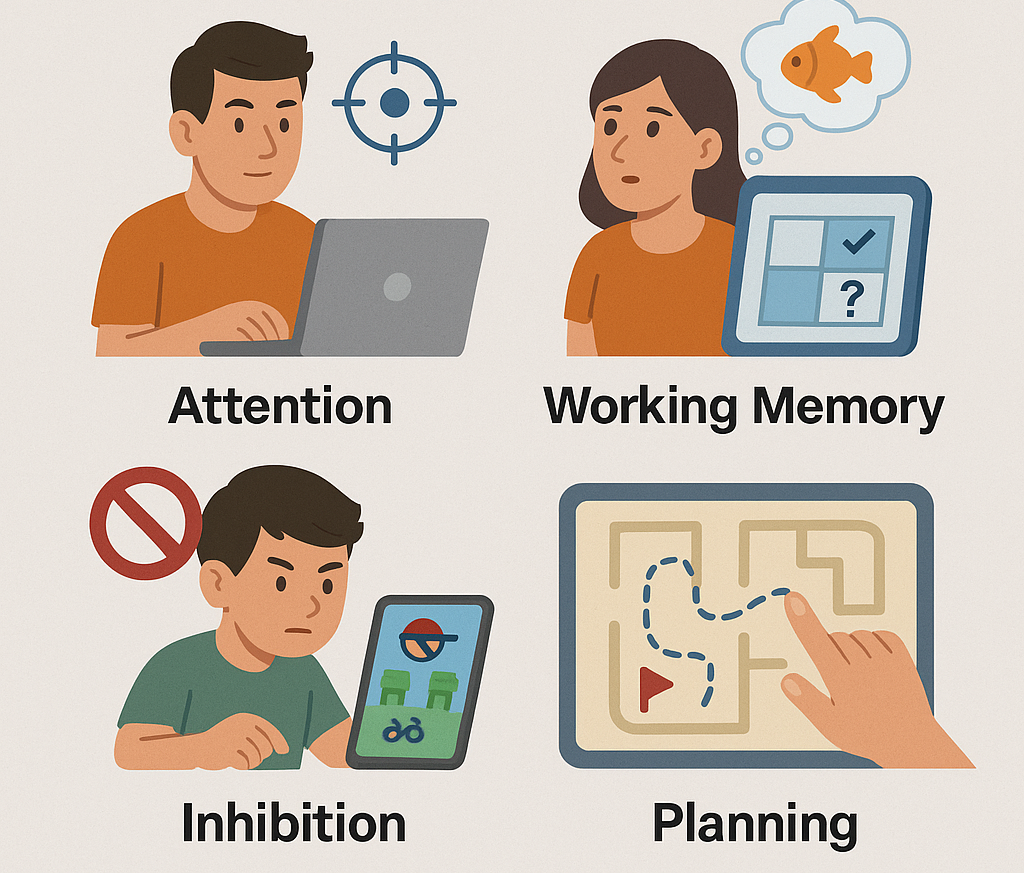
\includegraphics[width=1\textwidth]{Figures/cognitive.pdf}
 \caption{Core cognitive models targeted by serious games in ADHD interventions: attention, working memory, inhibition, and planning. Each model maps to a specific set of game dynamics and EEG markers.}
 \label{fig:cognitive_models}
\end{figure}



Serious games integrated with BCI technology have demonstrated therapeutic benefits by reinforcing executive function, improving behavioral outcomes, and reducing symptom severity through active attention training and neurofeedback mechanisms \cite{Doulou2025}. Active BCIs, in which users intentionally modulate their focus to influence the outcome of the game, have been shown to strengthen cognitive control and promote long-term neuroplastic changes relevant to ADHD pathology \cite{Cervantes2023}. These platforms also enable adaptive feedback, allowing interventions to dynamically adjust to each child's neurocognitive profile.

However, the effectiveness of such systems depends on precise temporal synchronization between game-generated stimuli and EEG signals. Detecting event-related potentials (such as the P300 wave) or dynamic oscillations in the theta and beta frequency bands during attentional tasks requires sub-millisecond timing accuracy \cite{Wikstrom2022, Sandstrak2024}. Without rigorous synchronization—typically achieved via TTL triggers or low-latency USB/Wi-Fi communication—EEG signal interpretation is susceptible to noise, jitter, and event misclassification \cite{iwama2023two}. This challenge is particularly critical in real-time therapeutic environments where accurate feedback is essential.

Recent developments in portable EEG hardware have expanded the applicability of BCIs for ADHD beyond clinical settings, enabling real-time monitoring and feedback in homes, classrooms, and therapeutic environments. Low-cost, wireless EEG headsets—equipped with dry electrodes and embedded microcontrollers—have been successfully integrated into neurofeedback systems and serious games designed for children \cite{Xu2018}. These platforms allow for real-time signal acquisition and onboard processing, supporting closed-loop interventions without reliance on external computers. Thanks to ARM-based processors and system-on-chip (SoC) designs, it is now possible to run lightweight machine learning models directly on the device for real-time EEG classification \cite{Wang_2020}. Moreover, custom head-mounted EEG systems have shown reliable tracking of the theta/beta ratio, a key biomarker for ADHD, during interactive tasks \cite{Larocco2020}.

Altogether, these technological advances offer a promising foundation for rethinking ADHD diagnosis and intervention—especially in child populations. Nevertheless, critical technical challenges remain, particularly the synchronization of cognitive stimuli with neurophysiological responses in embedded systems. This challenge motivates the present research, which aims to design and implement a portable EEG acquisition and analysis system with precise synchronization to game events, enabling objective, real-time support for cognitive stimulation and diagnostic processes in children with ADHD.








\section{Problem statement}
\label{sec:problem} 

The design and implementation of serious games synchronized with neurophysiological signals such as electroencephalography (EEG) presents a critical challenge, especially when targeting cognitive stimulation and diagnostic support in pediatric populations with Attention Deficit Hyperactivity Disorder (ADHD). The scientific validity of such applications is fundamentally dependent on the precise temporal synchronization of at least two disparate data streams: the high-temporal-resolution physiological data from the EEG system and the context-dependent event data generated by the serious game. A core technical obstacle lies in achieving this precise synchronization, a requirement that is essential for both the accuracy of event-related potential (ERP) measurements and the effectiveness of real-time interventions.1 This thesis addresses two primary facets of this challenge: the temporal inaccuracies introduced by system-level operations and the physical limitations of the hardware itself.

\subsection{Unpredictable Latency and Jitter Between Game Events and EEG Recordings}

The primary technical issue in synchronizing EEG data with serious game events is the presence of unpredictable latency and jitter.2
Latency is the delay between an event's physical occurrence (e.g., a stimulus appearing on screen) and its corresponding timestamp being recorded in the data stream. A more pernicious issue is jitter, defined as the statistical variability in that latency over time.4 While a constant latency might be correctable in post-processing, jitter introduces random, unpredictable timing errors that cannot be easily removed after data acquisition.
This issue is caused by several interrelated factors: buffering delays in data pipelines, the non-deterministic scheduling of non-real-time operating systems, variability in communication protocols (such as USB, Bluetooth, or the Lab Streaming Layer), and asynchronous execution within game engines like Unity.5 These conditions lead to a lack of temporal precision, where the timestamp of an in-game event does not accurately align with the corresponding entry in the EEG data stream.
This misalignment significantly compromises the quality of neurophysiological analysis. ERP components such as the P300 and N200, which are commonly used to evaluate attentional processes in ADHD, depend on millisecond-level synchronization between stimulus onset and neural response.7 When event markers are not precisely aligned due to jitter, the resulting ERP waveform becomes temporally "smeared," causing a reduction in both amplitude and interpretability, which degrades the signal-to-noise ratio and threatens diagnostic reliability.2 This is particularly critical in pediatric populations where subtle attentional deficits are being assessed.
Furthermore, in real-time systems like neurofeedback applications, where immediate feedback is essential for operant conditioning, even minor delays can disrupt the feedback loop. If the user receives auditory or visual feedback that no longer corresponds precisely to their brain state, the therapeutic effectiveness is reduced, potentially leading to user disengagement or ineffective training outcomes.2 The temporal precision required is demanding; some brain-computer interface (BCI) paradigms require accuracy within ±2 milliseconds, yet jitter introduced by a game's graphical rendering at 50 frames per second can be as high as 20 milliseconds.
Recent studies have quantified these challenges. For example, Larsen et al. (2024) found that even in systems optimized with Unity and LSL, event marker delays averaged 36 milliseconds with a jitter of 5 to 6 milliseconds—well above the acceptable margin for many ERP analyses.9 Additionally, Brain Products (2024) reports that embedded platforms lacking efficient buffering and timestamping can exhibit latencies up to 100 milliseconds, particularly under high computational load.5 These delays, caused by a lack of dedicated real-time scheduling and protocol optimization, result in a substantial loss of synchronization fidelity, ultimately undermining both research validity and clinical utility.


\subsection{Resource and power constraints in embedded EEG platforms}

The second major issue stems from the computational and energy limitations of embedded and wearable EEG systems. Designed to be mobile and unobtrusive, these systems often operate on limited battery power, constrained CPU cycles, and reduced memory.11 These constraints are exacerbated when the system must simultaneously support real-time data acquisition, multichannel EEG streaming, and high-frequency event marker registration. Conventional EEG setups that rely on centralized data processing can also lead to high energy consumption and increased data transmission latency.12
These limitations make it difficult to implement low-latency communication and high-resolution timestamping. Wireless data transmission, in particular, is very power-intensive.13 Protocols such as Bluetooth and Wi-Fi—commonly used in portable EEG systems—can introduce packet retransmissions, buffering delays, and inconsistent delivery times that worsen synchronization accuracy.5
The consequences are significant. System designers are forced to lower EEG sampling rates, simplify marker handling, or accept increased delays—all of which reduce the reliability of the collected data and the interactivity of the game.14 For example, a review of wearable EEG systems found that wireless devices consistently showed worse timing stability and synchronization performance compared to wired configurations, especially when embedded resources were under heavy computational load.
Brain Products (2024) corroborates these findings, warning that system performance degrades as channel count and sampling rate increase—conditions commonly required in clinical-grade EEG systems.5 This creates a fundamental trade-off: increasing signal fidelity and temporal resolution compromises system portability, while optimizing for mobility sacrifices diagnostic precision.
Therefore, a critical gap exists in establishing a robust methodology to reliably synchronize multimodal data streams from EEG systems and dynamic serious games with quantifiable, millisecond-level precision, while also operating within the power and resource constraints of embedded platforms. This thesis addresses the problem of ensuring the temporal integrity of these data streams to enable scientifically valid analysis of neuro-cognitive processes during gameplay.


%The design and implementation of serious games synchronized with neurophysiological signals such as EEG presents a critical challenge in the domain of embedded systems, especially when targeting cognitive stimulation and diagnostic support in pediatric populations with Attention Deficit Hyperactivity Disorder (ADHD). A core technical obstacle lies in achieving precise synchronization between in-game events and EEG signal acquisition, a requirement that is essential for both the accuracy of event-related potential (ERP) measurements and the effectiveness of real-time interventions.

% \section{Problem Statement}

% The integration of EEG acquisition systems with serious games for neurocognitive stimulation and ADHD diagnosis in children is gaining relevance due to its potential for real-time, objective assessment of brain activity. However, when such systems are deployed on embedded or mobile platforms, two critical technical challenges arise that compromise their effectiveness: (1) unpredictable latency and jitter between the game engine and the EEG recorder, and (2) the resource and power constraints inherent to embedded systems. Both issues severely affect the temporal precision required for capturing event-related potentials (ERPs) and delivering valid neurofeedback or cognitive training.

%\subsection{Unpredictable Latency and Jitter Between Game Events and EEG Recordings}

%One of the primary technical issues in synchronizing EEG data with serious game events is the presence of unpredictable latency and jitter during the transmission of event markers. This issue is caused by several interrelated factors: buffering delays in data pipelines, the non-deterministic scheduling of non-real-time operating systems, variability in communication protocols (such as USB CDC, Bluetooth, or Lab Streaming Layer), and asynchronous execution within game engines like Unity. These conditions lead to a lack of temporal precision, where the timestamp of an in-game event does not accurately align with the corresponding entry in the EEG data stream.

%As a consequence, this misalignment significantly compromises the quality of neurophysiological analysis. ERP components such as the P300 and N200, commonly used to evaluate attentional processes in ADHD, depend on millisecond-level synchronization between stimulus onset and neural response. When event markers are not precisely aligned due to jitter or latency, the resulting ERP waveform becomes temporally smeared, causing a reduction in both amplitude and interpretability \cite{iwama2022jitter}. This degradation affects diagnostic reliability, particularly in pediatric populations where subtle attentional deficits are being assessed.

%Another cause of latency variability stems from the processing demands of real-time systems. In neurofeedback applications, where immediate feedback is essential for operant conditioning, even minor delays in EEG–event synchronization can disrupt the feedback loop. As a consequence, the user receives auditory or visual feedback that no longer corresponds precisely to their brain state, thereby reducing the therapeutic effectiveness and potentially leading to user disengagement or ineffective training outcomes.

%Recent studies have further demonstrated the impact of these technical challenges. For example, \cite{larsen2024quantifying} found that even in systems optimized with Unity and LSL, event marker delays averaged 36 milliseconds, with jitter ranging from 5 to 6 milliseconds—well above the acceptable margin for ERP-based analyses. Additionally, \cite{brainproducts2024lsl} reports that embedded platforms lacking efficient buffering and timestamping mechanisms can exhibit latencies up to 100 milliseconds, particularly under high computational load or poorly configured data streams. These delays are caused by a lack of dedicated real-time scheduling and protocol optimization, and the resulting consequence is a substantial loss of synchronization fidelity—ultimately undermining both research validity and clinical utility.


%\subsection{Resource and power constraints in embedded EEG platforms}

%The second major issue stems from the computational and energy limitations typical of embedded EEG systems. These systems, designed to be mobile and unobtrusive, often operate on limited battery power, constrained CPU cycles, reduced memory, and variable wireless connectivity. These constraints are exacerbated when the system must support real-time data acquisition, multichannel EEG streaming, and high-frequency marker registration simultaneously.

%These limitations make it difficult to implement low-latency communication and high-resolution timestamping. In particular, wireless protocols such as Bluetooth and Wi-Fi—commonly used in portable EEG systems—introduce packet retransmissions, buffering delays, and inconsistent delivery times that worsen synchronization accuracy.

%The consequences are significant. System designers are forced to lower EEG sampling rates, simplify marker handling, or accept increased delays—all of which reduce the reliability of the collected data and the interactivity of the game. For example, \cite{liu2024fpga} reviewed wearable EEG systems and found that wireless devices consistently showed worse timing stability and synchronization performance compared to wired configurations, especially when embedded resources were under heavy computational load.

%\cite{brainproducts2024lsl} corroborates these findings, warning that system performance degrades as channel count and sampling rate increase—conditions commonly required in clinical-grade EEG systems. This creates a fundamental trade-off: increasing signal fidelity and temporal resolution compromises system portability, while optimizing for mobility sacrifices diagnostic precision.

\begin{figure}
    \centering
    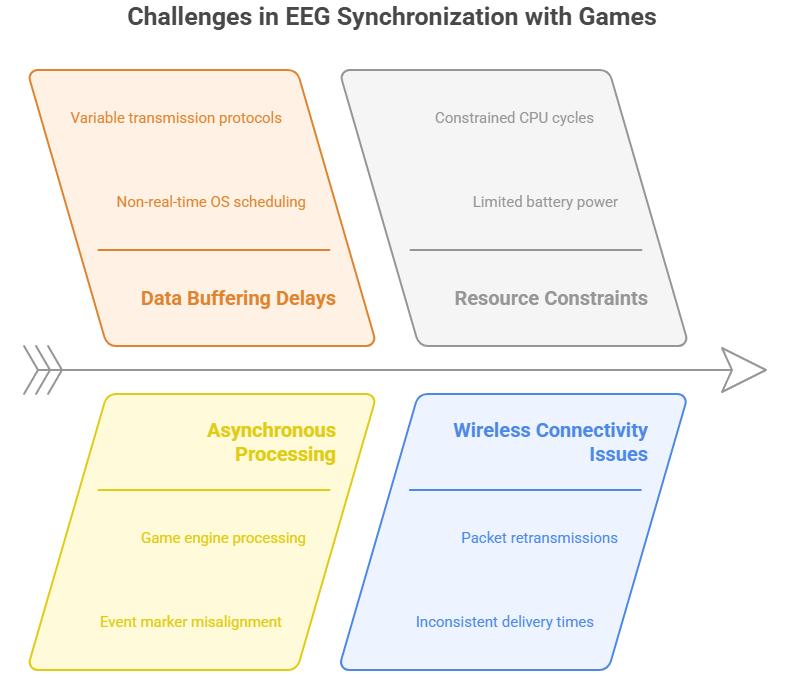
\includegraphics[width=0.8\linewidth]{Figures/state of the art.png}
    \caption{}
    \label{fig:Esquema}
\end{figure}

% In summary, the combined effects of latency/jitter and resource limitations in embedded EEG systems threaten the temporal accuracy and clinical reliability of serious games for ADHD evaluation. These challenges must be addressed to ensure that event markers in the game are precisely aligned with EEG recordings, and that the system can operate effectively in real-world, mobile, and child-friendly environments.





% \subsection{Lattency and jitter}

% One major subproblem is the presence of latency and jitter in the transmission of event markers from the game engine to the EEG recording system. Even under tightly controlled experimental setups, delays in marker delivery can vary significantly due to factors such as USB buffering, wireless transmission, and operating system scheduling. Recent studies report latency offsets averaging 36 ms with jitter exceeding 5 ms in Unity–LSL pipelines, which can distort ERP measurements and limit the effectiveness of closed-loop systems (Larsen et al., 2024). Moreover, Iwama et al. (2022) emphasize that even small jitters of ±5 ms are sufficient to degrade the temporal accuracy required for neurofeedback and ERP-based paradigms. Vendor documentation from Brain Products (2024) warns that such delays can reach up to 100 ms on low-power embedded devices unless buffering and sampling rates are carefully tuned.

% % \subsection{synchronization interface}

% % A second subproblem is the lack of standardized synchronization interfaces across the heterogeneous hardware and software components involved in EEG–game integration. Serious games, microcontrollers, and EEG amplifiers often utilize disparate protocols such as TTL pulses, USB CDC, BLE, and Lab Streaming Layer (LSL), each with its own timing architecture and limitations. Miziara et al. (2025) found that hardware-based triggers offered substantially greater timing accuracy than software-based LSL alternatives, though at the expense of system scalability. Similarly, commercial EEG systems such as Zeto WR19 can embed low-jitter markers via proprietary hardware, but still require complex reconciliation when integrating third-party devices through LSL or TTL (Zeto Inc., 2023). Brain Products (2024) highlights the risk of marker misalignment when synchronizing systems that rely on different timestamping strategies without a unified clock.

% \subsection{Resource and power constraints in mobile/embedded EEG platforms}


% A third subproblem arises from computational and power limitations in mobile or embedded EEG systems, which restrict the feasibility of implementing high-resolution, low-latency synchronization protocols. Mobile EEG devices often operate on limited battery capacity and rely on wireless communication, which introduces variable delays due to packet buffering and retransmission. Liu et al. (2024) observed that wireless EEG systems generally exhibit reduced temporal stability compared to their wired counterparts, especially under higher sampling rates or increased channel counts. Brain Products (2024) also notes that latency tends to increase with system load, further complicating efforts to achieve precise synchronization in portable scenarios.
% These synchronization challenges are particularly consequential in ADHD-focused applications, where the reliability of stimulus-locked EEG features such as the P300 or N200 components is crucial for diagnostic and therapeutic efficacy. Real-time adaptive feedback mechanisms—common in gamified neurofeedback interventions—require consistent round-trip latencies under 100 ms, while embedded systems deployed in schools or clinics must balance timing accuracy with constraints on power, cost, and usability. Addressing the issues of latency and jitter, protocol standardization, and resource optimization is thus vital for the development of robust and clinically useful EEG–game synchronization systems.


% Agregar las graficas del estado del arte 


\newpage
\section{Pregunta de investigación}\label{sec:question}

How can a low-latency and low-jitter data synchronization framework be developed and validated to ensure the temporal integrity of multimodal data from embedded EEG systems and dynamic serious game events, while respecting the inherent resource and power constraints of such platforms?



\section{Estado del arte}\label{sec:stateofart}


In recent years, numerous wireless systems for EEG data acquisition have been developed, with two main approaches standing out: conventional remote monitoring systems and portable smart systems. The former simply digitize the EEG signals and transmit them to a remote unit for processing, usually in a deferred manner \cite{arpaia2020wearable}. On the other hand, portable systems preprocess the signals on a local device, such as a microcontroller (MCU), and wirelessly transmit the data using low-power consumption protocols. \ref{table:bci_hardware} This latter approach is crucial for real-time applications, where low latency is essential.

Marker synchronization in portable EEG acquisition systems \cite{razavi2022opensync}, particularly in applications combined with serious games \cite{damavsevivcius2023serious}, faces several technical and operational challenges. One of the main issues lies in latency in data transmission protocols. In portable EEG systems, precise synchronization between brain events and interactions in the game is crucial \cite{gomezromero2024implications}, but inherent limitations of portable acquisition systems, such as latencies in data transfer protocols, can cause temporal mismatches. These latencies primarily stem from bandwidth constraints in wireless transmission and the need to process large volumes of data in real-time \cite{he2023diversity}.

The type of electrode \cite{liu2023feature} and the number of channels \cite{abdullah2022eeg}  are determining factors in the quality of the data acquired in portable systems. Although dry electrodes offer greater portability, they tend to generate lower-quality signals due to reduced conductivity, which can complicate precise synchronization with other devices, such as serious games. On the other hand, the use of systems with \textbf{low channel density (e.g., 8-16 channels)} \cite{allouch2023effect} is a common strategy in these portable systems to minimize size and improve portability. However, low channel density can affect the spatial resolution of EEG data, limiting the ability to perform accurate analysis of brain patterns. This challenge is reflected in the need to optimize sampling \cite{zheng2023effects}  and data transfer protocols \cite{bayilmics2022survey}  to ensure that captured signals are transmitted efficiently without significant information loss

The sampling rate is another critical factor, as it directly affects the temporal resolution of EEG signals. The combination of low channel density and insufficient sampling rate can make it difficult to capture fast brain events, such as attention shifts, which are essential in applications like serious games. Furthermore, Signal Front-End Amplifiers (AFE) \cite{devi2022survey} play a key role in signal quality. While low-cost AFEs may be suitable for portable systems, they tend to have limitations in processing capacity, which impacts data synchronization by generating noise and distortions in the EEG signals, especially when connected to mobile devices with lower processing power.

Battery life \cite{niso2023wireless} is a significant constraint for portable systems that require long monitoring sessions. EEG systems that operate for several hours often need to optimize their energy consumption, which may involve reducing the sampling rate or channel density, once again impacting data quality and real-time synchronization.


\begin{table}[H]
    \caption{Dispositivos de adquisición utilizados para BCI. La tabla ofrece una descripción general de los diferentes dispositivos de hardware, sus especificaciones y protocolos de comunicación.}
    \label{table:bci_hardware}
    \centering
    \begin{tabular}{|p{2cm}|p{1.5cm}|p{1.6cm}|p{1.6cm}|p{1.7cm}|p{1.4cm}|p{1.8cm}|p{1.4cm}|}
        \hline
        \textbf{Hardware BCI} & \textbf{Empresa} & \textbf{Tipo de Electrodo} & \textbf{Canales} & \textbf{Frecuencia de Muestreo} & \textbf{AFE} & \textbf{Protocolo y Transferencia de Datos} & \textbf{Duración de la Batería} \\ \hline
        Cyton + Daisy \cite{OpenBCI_CytonDaisy} & OpenBCI & Flexible / Húmedo / Seco & 16 & 250 Hz- -16 kHz & ADS1299 & RF / BLE / Wi-Fi & 8 h \\ \hline
        actiCAP \cite{BrainProducts_ActiCap} & Brain Products GmbH & Flexible / Húmedo / Seco & 16 & 256 Hz- -16 kHz & - & USB & 16 h \\ \hline
        EPOC X \cite{Emotiv_EPOCX} & Emotiv & Rígido / Húmedo & 14 & 128 Hz & - & BLE / Bluetooth & 6--12 h \\ \hline
        Diadem \cite{Bitbrain_Diadem} & Bitbrain & Rígido / Seco & 12 & 256 Hz & - & Bluetooth & 8 h \\ \hline
        g.Nautilus \cite{Gtec_GNautilusProFlexible} & g.tec & Flexible & 8 / 16 / 32 & 250 Hz & ADS1299 & Propietario & 10 h \\ \hline
        Plataforma para EEG ambulatorio \cite{pinho2014wireless} & - & Activo / Seco & 32 & 250 Hz- -1 kHz & ADS1299 & Wi-Fi 802.11 b/g/n & 26 h \\ \hline
        Sistema para neurofeedback \cite{Totev2023} & - & Pasivo / Seco & 40 & 250 Hz & ADS1298 & RF & - \\ \hline
        BEATS \cite{Beats} & - & Flexible / Húmedo & 32 & 4 kHz & ADS1299 & Wi-Fi & 24 h (cableado) \\ \hline
    \end{tabular}
\end{table}


% \begin{table}[H]
%     \caption{Acquisition devices used for BCI. The table provides an overview of different hardware devices, their specifications, and communication protocols.}
%     \label{table:bci_hardware}
    
% \begin{adjustwidth}{-\extralength}{0cm}
%         \setlength{\cellWidtha}{\fulllength/8-2\tabcolsep+0.6in}
%         \setlength{\cellWidthb}{\fulllength/8-2\tabcolsep-0.1in}
%         \setlength{\cellWidthc}{\fulllength/8-2\tabcolsep-0in}
%         \setlength{\cellWidthd}{\fulllength/8-2\tabcolsep-0in}
%         \setlength{\cellWidthe}{\fulllength/8-2\tabcolsep-0.2in}
%         \setlength{\cellWidthf}{\fulllength/8-2\tabcolsep-0.1in}
%         \setlength{\cellWidthg}{\fulllength/8-2\tabcolsep-0.1in}
%         \setlength{\cellWidthh}{\fulllength/8-2\tabcolsep-0.1in}
%         \scalebox{1}[1]{\begin{tabularx}{\fulllength}{
%                     >{\PreserveBackslash\centering}m{\cellWidtha}
%                     >{\PreserveBackslash\centering}m{\cellWidthb}
%                     >{\PreserveBackslash\centering}m{\cellWidthc}
%                     >{\PreserveBackslash\centering}m{\cellWidthd}
%                     >{\PreserveBackslash\centering}m{\cellWidthe}
%                     >{\PreserveBackslash\centering}m{\cellWidthf}
%                     >{\PreserveBackslash\centering}m{\cellWidthg}
%                     >{\PreserveBackslash\centering}m{\cellWidthh}}
%                 \toprule 
%                 \textbf{BCI Hardware} & \textbf{Company} & \textbf{Electrode Type} & \textbf{Channels} & \textbf{Sampling Rate} & \textbf{AFE} & \textbf{Protocol and Data Transfer} & \textbf{Battery Life} \\
%                 \midrule
%                 Cyton + Daisy \cite{OpenBCI_CytonDaisy} & OpenBCI & Flexible/Wet/Dry & 16 & 250 Hz--16 kHz & ADS1299 & RF/BLE/Wi-Fi & 8 h \\
%                 actiCAP\cite{BrainProducts_ActiCap} & Brain Products GmbH & Flexible/Wet/Dry & 16 & 256 Hz--16 kHz & - & USB & 16 h \\
                
%                 EPOC X \cite{Emotiv_EPOCX}& Emotiv & Rigid/Wet & 14 & 128 Hz & - & BLE/Bluetooth & 6--12 h \\
                
%                 Diadem \cite{Bitbrain_Diadem}& Bitbrain & Rigid/Dry & 12 & 256 Hz & - & Bluetooth & 8 h \\
                
%                 g.Nautilus \cite{Gtec_GNautilusProFlexible} & g.tec & Flexible & 8/16/32 & 250 Hz & ADS1299 & Proprietary & 10 h \\
                
%                 Platform for ambulatory EEG \cite{pinho2014wireless} & - & Active/Dry & 32 & 250 Hz--1 kHz & ADS1299 & Wi-Fi 802.11 b/g/n & 26 h \\
                
%                 System for neurofeedback \cite{Totev2023} & - & Passive/Dry & 40 & 250 Hz & ADS1298 & RF & - \\
                
%                 BEATS \cite{Beats} & - & Flexible/Wet & 32 & 4 kHz & ADS1299 & Wi-Fi & 24 h (wired) \\
%                 \bottomrule
%         \end{tabularx}}
%     \end{adjustwidth}
% \end{table}

In the field of brain-computer interfaces (BCIs), several devices have been developed, each with unique features tailored to specific use cases such as clinical research, neurofeedback, or consumer applications. The Cyton + Daisy system by OpenBCI \cite{OpenBCI_CytonDaisy} supports up to 16 channels and offers a wide sampling rate range of 250 Hz to 16 kHz, making it suitable for high-resolution EEG acquisition. The device uses flexible, wet, or dry electrodes and incorporates the ADS1299 AFE for high-quality signal conversion. It supports data transfer via RF, Bluetooth Low Energy (BLE), and Wi-Fi, allowing for versatile connectivity. With a battery life of 8 hours, this system is highly adaptable, suitable for both research and practical applications in various environments. Another system, actiCAP \cite{BrainProducts_ActiCap} by Brain Products GmbH, features flexible, wet, or dry electrodes and is capable of recording up to 16 channels with a sampling rate range from 256 Hz to 16 kHz. The actiCAP does not use a dedicated AFE and instead relies on a USB protocol for data transfer. The device provides a robust 16-hour battery life, making it an ideal choice for long-duration experiments and clinical settings that require stable signal acquisition over extended periods. The EPOC X \cite{Emotiv_EPOCX} by Emotiv is a more compact and consumer-oriented BCI device that uses rigid, wet electrodes and supports 14 channels with a sampling rate of 128 Hz. This device employs Bluetooth Low Energy (BLE) for wireless data transfer, and its battery life ranges from 6 to 12 hours, depending on usage. While its lower sampling rate may limit its use for high-resolution research, the EPOC X remains a popular choice for applications in neurofeedback, cognitive training, and general user interaction. The Diadem \cite{Bitbrain_Diadem} system by Bitbrain uses rigid, dry electrodes and supports 12 channels with a sampling rate of 256 Hz. It operates via Bluetooth for data transmission and has a battery life of 8 hours, providing a balance between portability and signal quality. The g.Nautilus \cite{Gtec_GNautilusProFlexible} system by g.tec offers great flexibility, supporting configurations with 8, 16, or 32 channels. It operates at a sampling rate of 250 Hz and uses the ADS1299 AFE for high-performance signal acquisition. The system is known for its proprietary data transmission protocol, ensuring reliable connectivity, and its battery lasts up to 10 hours, making it suitable for long-term monitoring and research studies. The BCI system used by \cite{pinho2014wireless} employs active, dry electrodes and supports up to 32 channels with a sampling rate range of 250 Hz to 1 kHz. It also incorporates the ADS1299 AFE for analog-to-digital conversion, ensuring high fidelity in signal capture. Data is transferred via Wi-Fi 802.11 b/g/n, enabling flexible and high-speed communication with external devices. The system boasts an impressive 26-hour battery life, making it an excellent option for extended usage in field studies or clinical applications. The BCI system described by \cite{Totev2023} uses passive, dry electrodes and supports up to 40 channels with a sampling rate of 250 Hz. It incorporates the ADS1298 AFE for high-quality data acquisition and utilizes RF (Radio Frequency) for data transfer. While battery life details are not specified, this device is likely designed for portable, research-focused applications where wireless data transfer is essential for real-time monitoring. Finally, the \cite{Beats} system features 32 flexible, wet electrodes and uses the ADS1299 AFE for high-precision EEG signal acquisition at a sampling rate of 4 kHz. Data is transmitted wirelessly via Wi-Fi, allowing for real-time data monitoring and analysis. The system’s battery life is 24 hours when wired, providing extended operation for intensive studies or clinical assessments that require continuous monitoring.

Each of these devices represents a different approach to EEG signal acquisition, offering varying numbers of channels, electrode types, sampling rates, and battery life. While some are optimized for research and clinical use with high sampling rates and extended battery life, others are more suited to consumer applications with lower sampling rates and shorter operational times. The choice of device depends largely on the specific needs of the user, whether for research, clinical monitoring, or personal use in neurofeedback and cognitive training applications.


% En los últimos años, se han desarrollado numerosos sistemas inalámbricos para la adquisición de datos EEG, destacándose dos enfoques principales: los sistemas convencionales de monitoreo remoto y los sistemas portátiles inteligentes. Los primeros simplemente digitalizan las señales EEG y las transmiten a una unidad remota para su procesamiento, generalmente de manera diferida \cite{arpaia2020wearable}. Por otro lado, los sistemas portátiles preprocesan las señales en un dispositivo local, como un microcontrolador (MCU), y transmiten los datos de manera inalámbrica utilizando protocolos de bajo consumo energético. \ref{table:bci_hardware} Este último enfoque es crucial para aplicaciones en tiempo real, donde la baja latencia es esencial.

% La duración de la batería \cite{niso2023wireless} es una restricción significativa para los sistemas portátiles que requieren sesiones de monitoreo largas. Los sistemas EEG que operan durante varias horas a menudo necesitan optimizar su consumo de energía, lo que puede implicar la reducción de la tasa de muestreo o la densidad de canales, lo que nuevamente impacta la calidad de los datos y la sincronización en tiempo real.

% La sincronización de marcadores en sistemas portátiles de adquisición de EEG \cite{razavi2022opensync}, particularmente en aplicaciones combinadas con juegos serios \cite{damavsevivcius2023serious}, enfrenta varios desafíos técnicos y operativos. Uno de los principales problemas radica en la latencia de los protocolos de transmisión de datos. En los sistemas portátiles de EEG, la sincronización precisa entre los eventos cerebrales y las interacciones en el juego es crucial \cite{gomezromero2024implications}, pero las limitaciones inherentes de los sistemas de adquisición portátiles, como las latencias en los protocolos de transferencia de datos, pueden causar desajustes temporales. Estas latencias provienen principalmente de las limitaciones de ancho de banda en la transmisión inalámbrica y la necesidad de procesar grandes volúmenes de datos en tiempo real \cite{he2023diversity}.

% El tipo de electrodo \cite{liu2023feature} y el número de canales \cite{abdullah2022eeg} son factores determinantes en la calidad de los datos adquiridos en los sistemas portátiles. Aunque los electrodos secos ofrecen mayor portabilidad, tienden a generar señales de menor calidad debido a la conductividad reducida, lo que puede complicar la sincronización precisa con otros dispositivos, como los juegos serios. Por otro lado, el uso de sistemas con \textbf{baja densidad de canales (por ejemplo, 8-16 canales)} \cite{allouch2023effect} es una estrategia común en estos sistemas portátiles para minimizar el tamaño y mejorar la portabilidad. Sin embargo, la baja densidad de canales puede afectar la resolución espacial de los datos EEG, limitando la capacidad para realizar un análisis preciso de los patrones cerebrales. Este desafío se refleja en la necesidad de optimizar la tasa de muestreo \cite{zheng2023effects} y los protocolos de transferencia de datos \cite{bayilmics2022survey} para asegurar que las señales capturadas se transmitan de manera eficiente sin pérdida significativa de información.

% La tasa de muestreo es otro factor crítico, ya que afecta directamente la resolución temporal de las señales EEG. La combinación de baja densidad de canales e insuficiente tasa de muestreo puede dificultar la captura de eventos cerebrales rápidos, como los cambios de atención, que son esenciales en aplicaciones como los juegos serios. Además, los amplificadores de señal front-end (AFE) \cite{devi2022survey} juegan un papel clave en la calidad de la señal. Si bien los AFE de bajo costo pueden ser adecuados para sistemas portátiles, tienden a tener limitaciones en capacidad de procesamiento, lo que impacta la sincronización de los datos al generar ruido y distorsiones en las señales EEG, especialmente cuando están conectados a dispositivos móviles con menor poder de procesamiento.  

% La duración de la batería \cite{niso2023wireless} es una restricción significativa para los sistemas portátiles que requieren sesiones de monitoreo largas. Los sistemas EEG que operan durante varias horas a menudo necesitan optimizar su consumo de energía, lo que puede implicar la reducción de la tasa de muestreo o la densidad de canales, lo que nuevamente impacta la calidad de los datos y la sincronización en tiempo real.

% \begin{table}[H]
%     \caption{Dispositivos de adquisición utilizados para BCI. La tabla ofrece una descripción general de los diferentes dispositivos de hardware, sus especificaciones y protocolos de comunicación.}
%     \label{table:bci_hardware}
%     \centering
%     \begin{tabular}{|p{2cm}|p{1.5cm}|p{1.6cm}|p{1.6cm}|p{1.7cm}|p{1.4cm}|p{1.8cm}|p{1.4cm}|}
%         \hline
%         \textbf{Hardware BCI} & \textbf{Empresa} & \textbf{Tipo de Electrodo} & \textbf{Canales} & \textbf{Frecuencia de Muestreo} & \textbf{AFE} & \textbf{Protocolo y Transferencia de Datos} & \textbf{Duración de la Batería} \\ \hline
%         Cyton + Daisy \cite{OpenBCI_CytonDaisy} & OpenBCI & Flexible / Húmedo / Seco & 16 & 250 Hz- -16 kHz & ADS1299 & RF / BLE / Wi-Fi & 8 h \\ \hline
%         actiCAP \cite{BrainProducts_ActiCap} & Brain Products GmbH & Flexible / Húmedo / Seco & 16 & 256 Hz- -16 kHz & - & USB & 16 h \\ \hline
%         EPOC X \cite{Emotiv_EPOCX} & Emotiv & Rígido / Húmedo & 14 & 128 Hz & - & BLE / Bluetooth & 6--12 h \\ \hline
%         Diadem \cite{Bitbrain_Diadem} & Bitbrain & Rígido / Seco & 12 & 256 Hz & - & Bluetooth & 8 h \\ \hline
%         g.Nautilus \cite{Gtec_GNautilusProFlexible} & g.tec & Flexible & 8 / 16 / 32 & 250 Hz & ADS1299 & Propietario & 10 h \\ \hline
%         Plataforma para EEG ambulatorio \cite{pinho2014wireless} & - & Activo / Seco & 32 & 250 Hz- -1 kHz & ADS1299 & Wi-Fi 802.11 b/g/n & 26 h \\ \hline
%         Sistema para neurofeedback \cite{Totev2023} & - & Pasivo / Seco & 40 & 250 Hz & ADS1298 & RF & - \\ \hline
%         BEATS \cite{Beats} & - & Flexible / Húmedo & 32 & 4 kHz & ADS1299 & Wi-Fi & 24 h (cableado) \\ \hline
%     \end{tabular}
% \end{table}

% En el campo de las interfaces cerebro-computadora (BCIs), se han desarrollado varios dispositivos, cada uno con características únicas adaptadas a casos de uso específicos como la investigación clínica, el neurofeedback o las aplicaciones para consumidores. El sistema Cyton + Daisy de OpenBCI \cite{OpenBCI_CytonDaisy} soporta hasta 16 canales y ofrece un amplio rango de tasa de muestreo de 250 Hz a 16 kHz, lo que lo hace adecuado para la adquisición de EEG de alta resolución. El dispositivo utiliza electrodos flexibles, húmedos o secos e incorpora el AFE ADS1299 para la conversión de señales de alta calidad. Soporta la transferencia de datos mediante RF, Bluetooth Low Energy (BLE) y Wi-Fi, lo que permite una conectividad versátil. Con una duración de batería de 8 horas, este sistema es altamente adaptable, adecuado tanto para la investigación como para aplicaciones prácticas en diversos entornos. Otro sistema, el actiCAP \cite{BrainProducts_ActiCap} de Brain Products GmbH, presenta electrodos flexibles, húmedos o secos y es capaz de grabar hasta 16 canales con un rango de tasa de muestreo de 256 Hz a 16 kHz. El actiCAP no utiliza un AFE dedicado, sino que depende de un protocolo USB para la transferencia de datos. El dispositivo proporciona una robusta duración de batería de 16 horas, lo que lo convierte en una opción ideal para experimentos de larga duración y entornos clínicos que requieren adquisición de señales estable a lo largo de períodos prolongados. El EPOC X \cite{Emotiv_EPOCX} de Emotiv es un dispositivo BCI más compacto y orientado al consumidor que utiliza electrodos rígidos y húmedos y soporta 14 canales con una tasa de muestreo de 128 Hz. Este dispositivo emplea Bluetooth Low Energy (BLE) para la transferencia de datos inalámbrica, y su duración de batería varía entre 6 y 12 horas, dependiendo del uso. Si bien su tasa de muestreo más baja puede limitar su uso para investigaciones de alta resolución, el EPOC X sigue siendo una opción popular para aplicaciones de neurofeedback, entrenamiento cognitivo e interacción general con el usuario. El sistema Diadem \cite{Bitbrain_Diadem} de Bitbrain utiliza electrodos rígidos y secos y soporta 12 canales con una tasa de muestreo de 256 Hz. Funciona mediante Bluetooth para la transmisión de datos y tiene una duración de batería de 8 horas, ofreciendo un equilibrio entre portabilidad y calidad de la señal. El sistema g.Nautilus \cite{Gtec_GNautilusProFlexible} de g.tec ofrece una gran flexibilidad, soportando configuraciones con 8, 16 o 32 canales. Opera a una tasa de muestreo de 250 Hz y utiliza el AFE ADS1299 para una adquisición de señales de alto rendimiento. El sistema es conocido por su protocolo de transmisión de datos propietario, que asegura una conectividad confiable, y su batería dura hasta 10 horas, lo que lo hace adecuado para monitoreo a largo plazo y estudios de investigación. El sistema BCI utilizado por \cite{pinho2014wireless} emplea electrodos activos y secos y soporta hasta 32 canales con un rango de tasa de muestreo de 250 Hz a 1 kHz. También incorpora el AFE ADS1299 para la conversión de señales analógicas a digitales, asegurando alta fidelidad en la captura de señales. Los datos se transfieren mediante Wi-Fi 802.11 b/g/n, lo que permite una comunicación flexible y de alta velocidad con dispositivos externos. El sistema presume una impresionante duración de batería de 26 horas, lo que lo convierte en una excelente opción para su uso prolongado en estudios de campo o aplicaciones clínicas. El sistema BCI descrito por \cite{Totev2023} utiliza electrodos pasivos y secos y soporta hasta 40 canales con una tasa de muestreo de 250 Hz. Incorpora el AFE ADS1298 para una adquisición de datos de alta calidad y utiliza RF (Radiofrecuencia) para la transferencia de datos. Aunque no se especifican detalles sobre la duración de la batería, este dispositivo está diseñado probablemente para aplicaciones portátiles y centradas en la investigación donde la transferencia inalámbrica de datos es esencial para el monitoreo en tiempo real. Finalmente, el sistema \cite{Beats} presenta 32 electrodos flexibles y húmedos y utiliza el AFE ADS1299 para una adquisición de señales EEG de alta precisión a una tasa de muestreo de 4 kHz. Los datos se transmiten de forma inalámbrica a través de Wi-Fi, lo que permite el monitoreo y análisis de datos en tiempo real. La duración de la batería del sistema es de 24 horas cuando está conectado por cable, lo que permite una operación extendida para estudios intensivos o evaluaciones clínicas que requieren monitoreo continuo.

% Cada uno de estos dispositivos representa un enfoque diferente para la adquisición de señales EEG, ofreciendo diversos números de canales, tipos de electrodos, tasas de muestreo y duración de batería. Mientras que algunos están optimizados para la investigación y el uso clínico con altas tasas de muestreo y larga duración de batería, otros son más adecuados para aplicaciones para consumidores con tasas de muestreo más bajas y tiempos de operación más cortos. La elección del dispositivo depende en gran medida de las necesidades específicas del usuario, ya sea para investigación, monitoreo clínico o uso personal en aplicaciones de neurofeedback y entrenamiento cognitivo.


\chapter{Aims}

\subsection{Objetivo General}
Diseñar e implementar una arquitectura de adquisición de señales EEG optimizada para aplicaciones en entornos educativos y clínicos, enfocada en la reducción de latencias y la sincronización precisa de eventos, para mejorar la evaluación objetiva de patrones cognitivos y emocionales en niños con TDAH.

\subsection{Objetivos Específicos}
\begin{enumerate}
    \item Analizar las limitaciones técnicas de los sistemas actuales de adquisición de EEG, incluyendo las latencias de transmisión y la baja densidad de canales.
    \item Desarrollar algoritmos de baja latencia y estrategias de sincronización temporal para garantizar la alineación precisa entre estímulos de juegos serios y respuestas EEG.
    \item Evaluar la arquitectura propuesta en entornos clínicos y educativos, verificando su eficacia en el diagnóstico y tratamiento del TDAH.
\end{enumerate}

\chapter{Outline and Contributions}
In this section, we provide a brief overview of the key contributions presented in this thesis, summarized in Figure \ref{fig:contributions}.
%\gls*{RFF} 

\begin{figure}[h!]
    \centering
    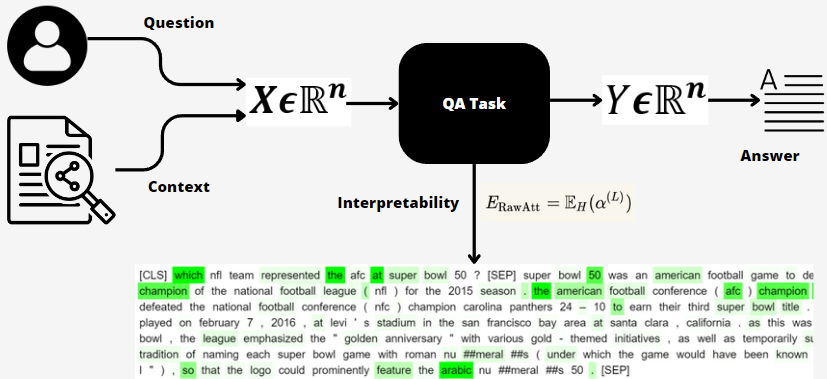
\includegraphics[width=1\linewidth,height=10cm]{Figures/outline_and_contributions/contributions.png}
    \caption[Scheme of an EQA task, illustrating the main contribution of this thesis, which allows finding the most relevant tokens to provide a precise answer to the question asked by the user.}
    \label{fig:contributions}
\end{figure}

This work contributes to the understanding of how transformer architectures work internally in the EQA task, based on the RawAtt \cite{abnar2020quantifying} interpretability technique, which allows finding the most relevant tokens of the context when answering a question made by the user. Our hybrid model represents a significant advance in interpretability by offering a clearer and more consistent interpretation of the results, paving the way for future research in this field.






\section{Arquitectura}

\begin{itemize}

    \item{Descripción General}

MindWave es un sistema avanzado diseñado para la adquisición y procesamiento de señales electroencefalográficas (EEG), con un diseño modular y escalable. Este sistema consta de varios módulos interconectados que aseguran una alta precisión en la captura de datos, estabilidad durante el proceso de adquisición y flexibilidad para su aplicación en investigación y diagnóstico clínico. Los electrodos, posicionados según el sistema 10-20, capturan señales eléctricas del cerebro y las transmiten a un módulo de conversión analógica a digital. Posteriormente, estas señales digitalizadas son gestionadas por un microcontrolador, que no solo regula el flujo de datos, sino que también monitorea la calidad de las señales adquiridas. Finalmente, el sistema se conecta a una plataforma de software que permite la visualización en tiempo real, el almacenamiento seguro de datos en servicios en la nube y la sincronización precisa con los eventos experimentales, facilitando así el análisis posterior, como se muestra en la figura \ref{fig:Esquema}.

\begin{figure}
    \centering
    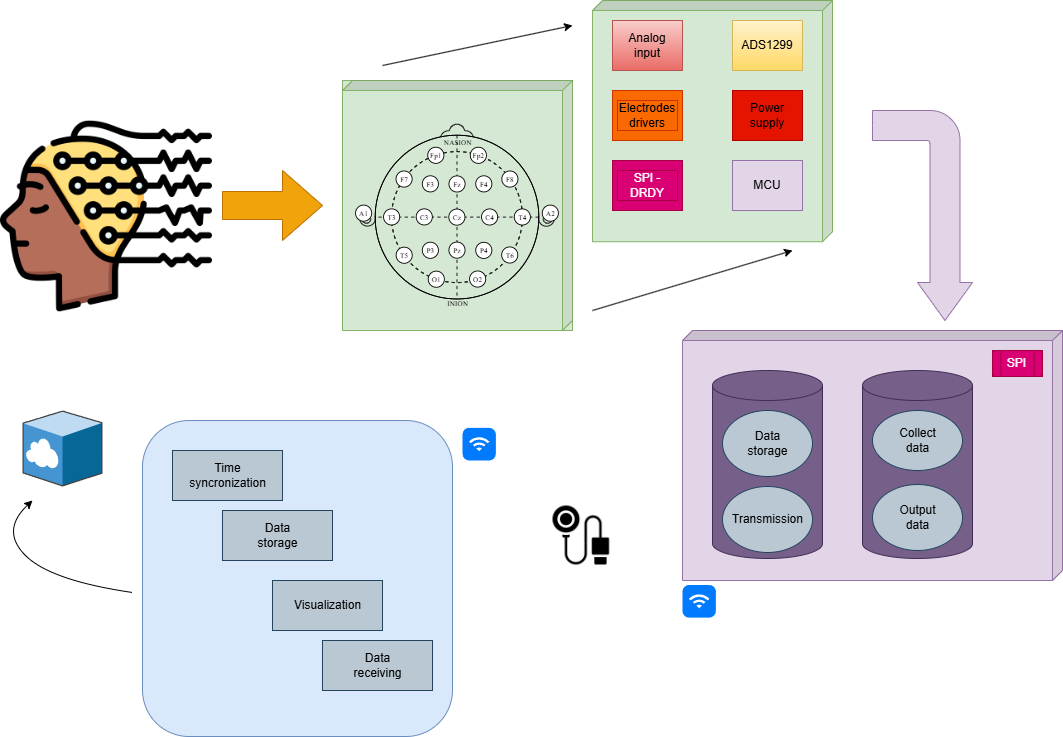
\includegraphics[width=0.8\linewidth]{Figures/DBP.png}
    \caption{Arquitectura de MindWave}
    \label{fig:Esquema}
\end{figure}

    \item {Módulo de Transmisión}

El módulo de transmisión de MindWave sirve como el centro neurálgico que conecta la adquisición de señales con su procesamiento y visualización externa. Consiste en varios subsistemas clave que operan de manera cohesionada:

    \item Módulo de Conversión Analógico-Digital

En el núcleo del módulo de adquisición se encuentra el ADS1299 de Texas Instruments \cite{TI_ADS1299}, un convertidor analógico-digital (ADC) de alta precisión diseñado específicamente para aplicaciones de monitoreo biológico como EEG, EMG y ECG. Este ADC presenta características que lo hacen ideal para capturar señales de baja amplitud, típicas de la actividad cerebral, como una resolución de 24 bits y un alto rango dinámico capaz de detectar variaciones sutiles en la actividad cerebral.

El ADS1299 incluye múltiples canales de entrada que pueden operar simultáneamente, lo que permite una adquisición de datos sincronizada. Además, tiene filtros digitales incorporados, como filtros pasa-bajo y notch, que ayudan a reducir el ruido y mejorar la relación señal-ruido antes de que las señales sean digitalizadas. Su capacidad para trabajar en configuraciones en cascada permite conectar hasta ocho módulos ADS1299, lo que soporta configuraciones de adquisición de datos de hasta 64 canales. Esto es esencial para estudios avanzados que requieren una cobertura amplia y detallada de la actividad cerebral.

    \item Transmisor

El sistema de transmisión de MindWave está diseñado para garantizar una transferencia rápida y confiable de los datos digitalizados a un dispositivo externo, como una computadora o servidor. Emplea un sistema de comunicación serial de alta velocidad, utilizando protocolos como UART o SPI, optimizados para minimizar la latencia durante la transmisión. Este enfoque asegura que los datos adquiridos puedan ser procesados o visualizados en tiempo real sin retrasos o pérdidas significativas, lo cual es crítico para aplicaciones que requieren una sincronización precisa, como experimentos en neurociencia o estudios clínicos con estimulación sincronizada.

Para asegurar conexiones eficientes y adaptables, el sistema puede integrar conversores USB-a-serial, lo que permite la compatibilidad con computadoras modernas sin interfaces seriales nativas. Además, MindWave puede incorporar transmisores inalámbricos, como módulos Bluetooth o Wi-Fi, para situaciones donde la movilidad o la eliminación de cables sea crucial. Sin embargo, la arquitectura inicial se centra en interfaces seriales por cable para priorizar la baja latencia y estabilidad.

    \item Microcontrolador

El microcontrolador elegido para MindWave debe manejar un alto volumen de datos provenientes de hasta 64 canales de EEG simultáneamente, además de supervisar los procesos de adquisición y comunicación. Una opción adecuada es el STM32H7 de STMicroelectronics \cite{STMicroelectronics_STM32H7}, basado en un núcleo ARM Cortex-M7. Este microcontrolador combina un rendimiento excepcional con una memoria RAM amplia y capacidades de procesamiento en tiempo real.

El STM32H7 incluye múltiples interfaces de comunicación, como SPI, I2C y UART, lo que permite la integración directa con los módulos ADS1299 y de transmisión. Su capacidad para manejar tareas paralelas asegura que pueda controlar múltiples módulos ADS1299 en configuraciones en cascada, gestionar la transmisión de datos a dispositivos externos y realizar operaciones de preprocesamiento básico, como detección de artefactos o validación de datos.

Además, su soporte para módulos de comunicación inalámbrica, incluyendo BLE y Wi-Fi, lo hace adaptable para futuras expansiones del sistema. Esto asegura que MindWave no solo cumpla con los requisitos actuales de adquisición, sino que también sea escalable para necesidades futuras.

    \item Software

La plataforma de software de MindWave está diseñada como una herramienta integral que proporciona visualización, almacenamiento y análisis de los datos de EEG. Esta plataforma, desarrollada con una interfaz gráfica amigable, permite a los investigadores y usuarios clínicos monitorear señales EEG en tiempo real con representaciones gráficas interactivas, incluyendo visualizaciones del espectro de frecuencias, tendencias temporales y patrones espaciales.

El software también se conecta a servicios de almacenamiento en la nube, lo que permite la copia de seguridad automática de los datos adquiridos y su accesibilidad para análisis remotos. Esta funcionalidad es esencial para proyectos colaborativos o investigadores que necesitan acceso a los datos desde diferentes ubicaciones geográficas.

Además de las características de visualización, la plataforma incluye un sistema de sincronización temporal que permite registrar eventos experimentales y asociarlos con las señales EEG correspondientes. Esto es particularmente útil en estudios que combinan estimulación visual o auditiva, ya que facilita la identificación de respuestas cerebrales específicas ante estímulos dados.

Las futuras implementaciones del software planean incluir herramientas de análisis automatizado basadas en inteligencia artificial, lo que permitirá a los investigadores identificar patrones complejos en los datos de EEG y generar informes detallados automáticamente.

\end{itemize}


\section{Materiales y Métodos}



El estudio fue diseñado para evaluar el rendimiento y las capacidades del sistema MindWave en un paradigma de juego serio orientado a la evaluación de procesos cognitivos mediante la adquisición de datos EEG. El hardware del sistema integra el convertidor analógico-digital (ADC) ADS1299 de Texas Instruments, que proporciona una adquisición de señales de alta resolución, y un microcontrolador capaz de encadenar múltiples ADCs para soportar hasta 64 canales EEG. Se utilizaron electrodos flexibles húmedos para registrar las señales electrofisiológicas, garantizando una recolección de datos confiable y al mismo tiempo asegurando la comodidad del participante durante sesiones de grabación extendidas. La transmisión de datos se implementó mediante un protocolo de comunicación serial, optimizado para minimizar la latencia y asegurar una transferencia de datos estable y en tiempo real a una computadora externa.

La plataforma de software desarrollada para el sistema permite la visualización en tiempo real, el almacenamiento y la gestión de los datos EEG. Esta plataforma también está integrada con un servicio de almacenamiento basado en la nube para el análisis posterior y la retención de datos a largo plazo. Además, el software facilita la presentación de estímulos visuales y auditivos a los participantes, asegurando una sincronización precisa entre las señales EEG y los eventos experimentales mediante registros con marcas de tiempo. Esta sincronización permite un análisis detallado de las respuestas cerebrales a eventos específicos del juego.
\chapter{Final Remarks}
\label{ch:chapter_5}


%======================================================================
\section{Conclusions}

In this research, we have addressed the crucial challenge of interpretability in question answering systems, especially in transformer-based architectures. Through the exhaustive evaluation of interpretability techniques and LLMs based on transformer architectures on the VisualMRC \cite{tanaka2021visualmrc} database, we have been able to propose a hybrid model that effectively combines the strengths of multiple LLMs and the RawAtt interpretability technique, demonstrating significant improvements in interpretability and robustness with respect to individual models.

On the other hand, our research provides a detailed comparison of RawAtt \cite{abnar2020quantifying}, AttCat \cite{qiang2022attcat} and Rollout \cite{abnar2020quantifying} interpretability techniques on transformer architectures such as BERT \cite{devlin2018bert}, Roberta \cite{liu2019roberta} and Distilbert \cite{sanh2019distilbert} on the VisualMRC database \cite{tanaka2021visualmrc}. The results reveal that RawAtt \cite{abnar2020quantifying} stands out as the most effective technique to improve interpretability in the EQA task on the VisualMRC database \cite{tanaka2021visualmrc}, offering a clearer understanding of the decision-making process in all the evaluated semantic classes of the VisualMRC database \cite{tanaka2021visualmrc}.

This research represents a significant advance in the understanding of how transformer architectures work internally in the EQA task, highlighting the importance of interpretability to improve confidence in the results and facilitate future research in this field.

\newpage


\section{Future Work}

To advance our research and build upon our current findings, we have identified
several directions for future work. The following are the next possible continuing paths we envision:

\begin{itemize}
    \item develop and implement a chatbot for the National University of Colombia - Manizales Campus. This will involve integrating the proposed hybrid model, as well as the identified interpretability techniques, into the question answering system. Extensive testing will be essential to ensure that the chatbot provides accurate and useful answers to university documentation queries.
    
    \item Improving the performance of transformer architectures in question answering (QA), machine reading comprehension (MRC), visual question answering (VQA) and visual machine reading comprehension (VMRC) tasks.

    \item Development new interpretability techniques at the token relevance level for transformer architecture in multiples NLP tasks.
    \end{itemize}

%\chapter{Appendix}


\section{MONELIB: BIBLIOTECA PARA COMUNICACIÓN SISTEMA EMBEBIDO-VIDEOJUEGO}

\label{apendice:monelib}

\textbf{Descripción}: La librería MoneLib permite establecer una comunicación eficiente entre videojuegos desarrollados en Unity y un sistema embebido externo. Su función principal es la captura en tiempo real de eventos de interacción dentro del videojuego, los cuales son codificados en formato hexadecimal y enviados vía USB para su posterior análisis y procesamiento en hardware embebido.


\begin{itemize}
    \item[\textbf{Versión}:] 1.0 (Mayo 2025)
    
    \item[\textbf{Componentes}:]
    
     \begin{itemize}
        \item \textbf{MoneLibrary.cs}: Clase que inicializa la librería nativa de Android en Unity y proporciona métodos para la gestión del driver y el envío de datos.
        \item \textbf{monelib-release.aar}: Librería nativa de Android responsable de la comunicación USB.
        \item \textbf{AndroidManifest.xml}: Archivo de configuración que define los permisos de USB y las actividades necesarias para la operación.
    \end{itemize}
\end{itemize}



\section{Requerimientos del Sistema}
\begin{itemize}
    \item[\textbf{Unity}:] Versión 6000.0.45f1 o superior.
    \item[\textbf{Sistema Operativo}:] Android 12 (Snow Cone) o superior.
    \item[\textbf{Hardware}:] Dispositivo Android con soporte para USB-C Host.
    \item[\textbf{Microcontrolador}:] Un microcontrolador que sea compatible con un periférico USB en modo \textit{device}.
\end{itemize}

\section*{Instalación y Configuración}
\begin{enumerate}
    \item \textbf{Importar Librería}: Colocar el archivo \texttt{monelib-release.aar} en el directorio \texttt{Assets/Plugins/Android} del proyecto en Unity.
    \item \textbf{Agregar Clase}: Ubicar el script \texttt{MoneLibrary.cs} en la carpeta de \texttt{Scripts} del proyecto.
    \item \textbf{Modificar el Manifest}: Incluir los siguientes permisos y características en el archivo \texttt{AndroidManifest.xml}:
    \begin{verbatim}
<uses-feature android:name="android.hardware.usb.host" />
<uses-permission android:name="android.permission.USB_PERMISSION" />
    \end{verbatim}
    \item \textbf{Inicializar el Plugin}: En el método \texttt{Start()} de un objeto principal (ej. \texttt{GameStartup.cs}), llamar a la función de inicialización: \\
    \texttt{MoneLibrary.InitializePlugin("com.beepro.monelib.PluginInstance");}
\end{enumerate}

\section*{Descripción de Funcionalidades}
\subsection*{Inicialización del Plugin}
\begin{itemize}
    \item[\textbf{Método}:] \texttt{InitializePlugin(string pluginName)}.
    \item[\textbf{Acción}:] Este método obtiene una referencia a la actividad actual de Unity, crea una instancia del plugin de Android y pasa el contexto de la actividad al plugin nativo para establecer la comunicación.
\end{itemize}

\subsection*{Envío de Datos por USB}
\begin{itemize}
    \item[\textbf{Método}:] \texttt{SendUsbData(sbyte a)}.
    \item[\textbf{Acción}:] Invoca el método nativo \texttt{sendUsbData} de la librería de Android para transmitir un evento, codificado como un entero \texttt{sbyte}.
\end{itemize}

\subsection*{Eventos Configurados}
La librería está preconfigurada para manejar los siguientes eventos de juego:

\begin{table}[h!]
\centering
\begin{tabular}{|l|c|c|}
\hline
\textbf{Evento} & \textbf{Código Decimal} & \textbf{Código Hexadecimal} \\ \hline
Jugador marca "O" & 0 & 0x00 \\ \hline
Jugador marca "X" & 1 & 0x01 \\ \hline
Reinicio del juego & -1 & 0xFF \\ \hline
\end{tabular}
\caption{Tabla de eventos configurados en MoneLib.}
\label{tab:eventos_monelib}
\end{table}

\section*{Ejemplo de Integración}
El siguiente fragmento de código ilustra cómo enviar eventos desde el videojuego:

\begin{lstlisting}[language=CSharp, caption={Ejemplo de implementación de envío de eventos.}, label={code:monelib_example}]
void OnCellClick(CellEnum content)
{
    if (content == CellEnum.Cross)
    {
        MoneLibrary.SendUsbData(1); // Evento para "X"
    }
    else if (content == CellEnum.Zero)
    {
        MoneLibrary.SendUsbData(0); // Evento para "O"
    }
}

void OnRestartButtonClick()
{
    MoneLibrary.SendUsbData(-1); // Evento de reinicio
}
\end{lstlisting}

\section*{Consideraciones de Seguridad}
\begin{itemize}
    \item Se debe verificar que la aplicación solicite los permisos USB correctamente cuando se conecte al sistema embebido.
    \item Para prevenir la sobresaturación del canal de comunicación, se recomienda mantener un intervalo mínimo de 1 milisegundo entre el envío de eventos consecutivos.
\end{itemize}

%Inicio del apéndice o anexos
% \begin{appendix}
% \chapter{Appendix}


\section{MONELIB: BIBLIOTECA PARA COMUNICACIÓN SISTEMA EMBEBIDO-VIDEOJUEGO}

\label{apendice:monelib}

\textbf{Descripción}: La librería MoneLib permite establecer una comunicación eficiente entre videojuegos desarrollados en Unity y un sistema embebido externo. Su función principal es la captura en tiempo real de eventos de interacción dentro del videojuego, los cuales son codificados en formato hexadecimal y enviados vía USB para su posterior análisis y procesamiento en hardware embebido.


\begin{itemize}
    \item[\textbf{Versión}:] 1.0 (Mayo 2025)
    
    \item[\textbf{Componentes}:]
    
     \begin{itemize}
        \item \textbf{MoneLibrary.cs}: Clase que inicializa la librería nativa de Android en Unity y proporciona métodos para la gestión del driver y el envío de datos.
        \item \textbf{monelib-release.aar}: Librería nativa de Android responsable de la comunicación USB.
        \item \textbf{AndroidManifest.xml}: Archivo de configuración que define los permisos de USB y las actividades necesarias para la operación.
    \end{itemize}
\end{itemize}



\section{Requerimientos del Sistema}
\begin{itemize}
    \item[\textbf{Unity}:] Versión 6000.0.45f1 o superior.
    \item[\textbf{Sistema Operativo}:] Android 12 (Snow Cone) o superior.
    \item[\textbf{Hardware}:] Dispositivo Android con soporte para USB-C Host.
    \item[\textbf{Microcontrolador}:] Un microcontrolador que sea compatible con un periférico USB en modo \textit{device}.
\end{itemize}

\section*{Instalación y Configuración}
\begin{enumerate}
    \item \textbf{Importar Librería}: Colocar el archivo \texttt{monelib-release.aar} en el directorio \texttt{Assets/Plugins/Android} del proyecto en Unity.
    \item \textbf{Agregar Clase}: Ubicar el script \texttt{MoneLibrary.cs} en la carpeta de \texttt{Scripts} del proyecto.
    \item \textbf{Modificar el Manifest}: Incluir los siguientes permisos y características en el archivo \texttt{AndroidManifest.xml}:
    \begin{verbatim}
<uses-feature android:name="android.hardware.usb.host" />
<uses-permission android:name="android.permission.USB_PERMISSION" />
    \end{verbatim}
    \item \textbf{Inicializar el Plugin}: En el método \texttt{Start()} de un objeto principal (ej. \texttt{GameStartup.cs}), llamar a la función de inicialización: \\
    \texttt{MoneLibrary.InitializePlugin("com.beepro.monelib.PluginInstance");}
\end{enumerate}

\section*{Descripción de Funcionalidades}
\subsection*{Inicialización del Plugin}
\begin{itemize}
    \item[\textbf{Método}:] \texttt{InitializePlugin(string pluginName)}.
    \item[\textbf{Acción}:] Este método obtiene una referencia a la actividad actual de Unity, crea una instancia del plugin de Android y pasa el contexto de la actividad al plugin nativo para establecer la comunicación.
\end{itemize}

\subsection*{Envío de Datos por USB}
\begin{itemize}
    \item[\textbf{Método}:] \texttt{SendUsbData(sbyte a)}.
    \item[\textbf{Acción}:] Invoca el método nativo \texttt{sendUsbData} de la librería de Android para transmitir un evento, codificado como un entero \texttt{sbyte}.
\end{itemize}

\subsection*{Eventos Configurados}
La librería está preconfigurada para manejar los siguientes eventos de juego:

\begin{table}[h!]
\centering
\begin{tabular}{|l|c|c|}
\hline
\textbf{Evento} & \textbf{Código Decimal} & \textbf{Código Hexadecimal} \\ \hline
Jugador marca "O" & 0 & 0x00 \\ \hline
Jugador marca "X" & 1 & 0x01 \\ \hline
Reinicio del juego & -1 & 0xFF \\ \hline
\end{tabular}
\caption{Tabla de eventos configurados en MoneLib.}
\label{tab:eventos_monelib}
\end{table}

\section*{Ejemplo de Integración}
El siguiente fragmento de código ilustra cómo enviar eventos desde el videojuego:

\begin{lstlisting}[language=CSharp, caption={Ejemplo de implementación de envío de eventos.}, label={code:monelib_example}]
void OnCellClick(CellEnum content)
{
    if (content == CellEnum.Cross)
    {
        MoneLibrary.SendUsbData(1); // Evento para "X"
    }
    else if (content == CellEnum.Zero)
    {
        MoneLibrary.SendUsbData(0); // Evento para "O"
    }
}

void OnRestartButtonClick()
{
    MoneLibrary.SendUsbData(-1); // Evento de reinicio
}
\end{lstlisting}

\section*{Consideraciones de Seguridad}
\begin{itemize}
    \item Se debe verificar que la aplicación solicite los permisos USB correctamente cuando se conecte al sistema embebido.
    \item Para prevenir la sobresaturación del canal de comunicación, se recomienda mantener un intervalo mínimo de 1 milisegundo entre el envío de eventos consecutivos.
\end{itemize}%
% \end{appendix}

%Permite visualizar la bibliografía en la tabla de contenido
\addcontentsline{toc}{chapter}{Referencias} %Literatura Citada

\let\OLDthebibliography=\thebibliography
\def\thebibliography#1{\OLDthebibliography{#1}}
{
%\scriptsize % Comenta o elimina esta línea para volver al tamaño de fuente normal
\normalsize % O añade esto si quieres asegurarte de que es el tamaño normal
%\pagestyle{plain}
\bibliographystyle{dtvstyle}
% Nombre del documento donde se almacenan las referencias
\bibliography{Julian/References}
\nocite{*}
\cleardoublepage
}


\end{document}